\section{Aim}
 To study joins, set operations, nested queries, and grouping using the GROUP BY keyword.

\section{{Theory}}

\subsection{Joins}

The PostgreSQL Joins clause is used to combine records from two or more tables in a database. A JOIN is a means for combining fields from two tables by using values common to each.

\subsection{Set Operations}

Set operations include:
\begin{itemize}
	\item UNION: The UNION operator combines result sets of two or more SELECT statements into a single result set. Both the tables must have the same number of coulumns, and the corresponding columns must have compatible data types.
	\item INTERSECT: The INTERSECT operator also combines the result sets of two or more SELECT statements into a single result set. The INTERSECT operator returns any rows that are available in both result set or returned by both queries.
	\item EXCEPT: The EXCEPT operator returns distinct rows from the first query that are not in the output of the second query
\end{itemize}

\subsection{Nested Queries}

Nested query is a query within another PostgreSQL query and are usually embedded within the WHERE clause.\newline
A subquery is used to return data that will be used in the main query as a condition to further restrict the data to be retrieved.\newline
Subqueries can be used with the SELECT, INSERT, UPDATE and DELETE statements along with the operators like $=, <, >, >=, <=$, IN, etc.

\subsubsection{Example Syntax}


\begin{minted}{sql}
SELECT column_name [, column_name ]
FROM   table1 [, table2 ]
WHERE  column_name OPERATOR
      (SELECT column_name [, column_name ]
      FROM table1 [, table2 ]
      [WHERE]);
\end{minted}

\subsection{Grouping}

The GROUP BY clause is used to group the result table on the basis of one or more rows. This can be used in conjunction with Aggregate functions to display aggregate outputs.

\subsubsection{Syntax}

\begin{minted}{sql}
SELECT <colulmns> FROM <table>
	[WHERE <condition>]
	GROUP BY <column1>[, <column2>, ...];
\end{minted}

\section{{Code and Output}}

\subsubsection{Tables and their schemas}

\subsubsection{Items}
itemid (primary key)\newline
itemname\newline
category\newline
price\newline
instock\newline

\subsubsection{Customers}
custid (primary key)\newline
custname\newline
address\newline
state\newline

\subsubsection{Orders}
orderid (primary key)\newline
itemid\newline
quantity\newline
orderdate\newline

\subsubsection{Delivery}
delivery id (primary key)\newline
custid\newline
orderid\newline

\newline
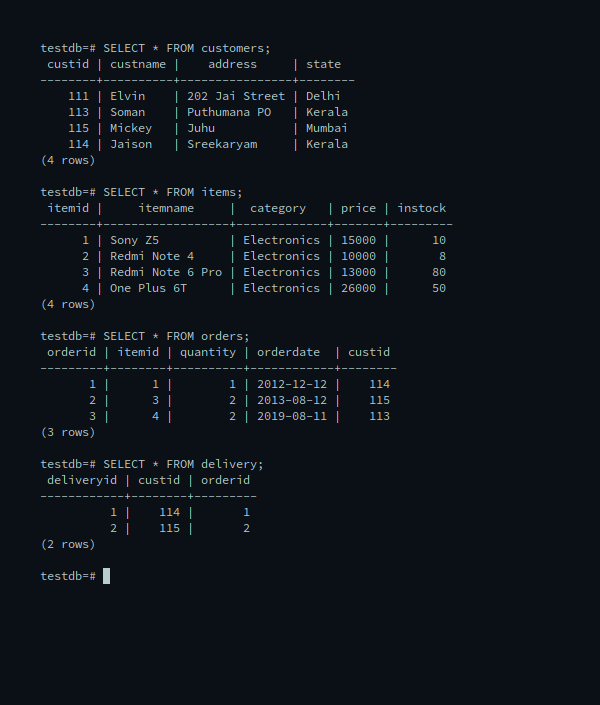
\includegraphics[width=\linewidth]{../Images/Joins/tables.png}

\begin{enumerate}
\item List the details of all customers who have placed an order\newline
\begin{minted}{sql}

SELECT * FROM customers WHERE custid IN 
	(SELECT custid FROM orders);

\end{minted}
\newline
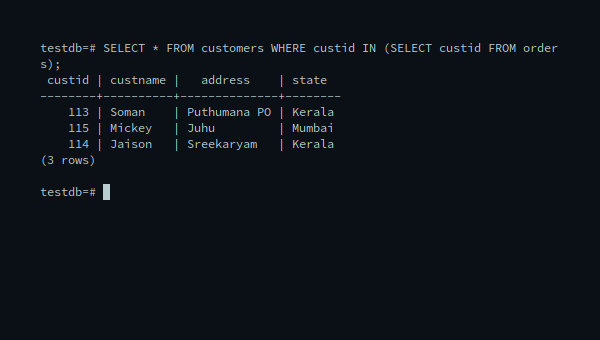
\includegraphics[width=\linewidth]{../Images/Joins/1.png}
\item List the details of all customers whose orders have been delivered\newline
\begin{minted}{sql}

SELECT * FROM customers WHERE custid IN 
	(SELECT custid FROM delivery);

\end{minted}
\newline
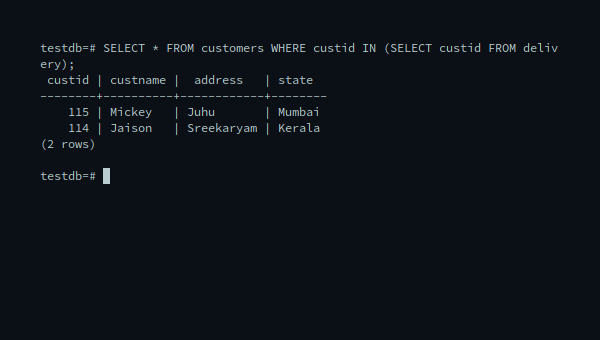
\includegraphics[width=\linewidth]{../Images/Joins/2.png}
\item Find the orderdate for all customers whose name starts in the letter ‘J’\newline
\begin{minted}{sql}

SELECT orderdate FROM orders WHERE EXISTS 
    (SELECT custname FROM customers 
        WHERE customers.custid = orders.custid AND 
              custname LIKE 'J%');

\end{minted}
\newline
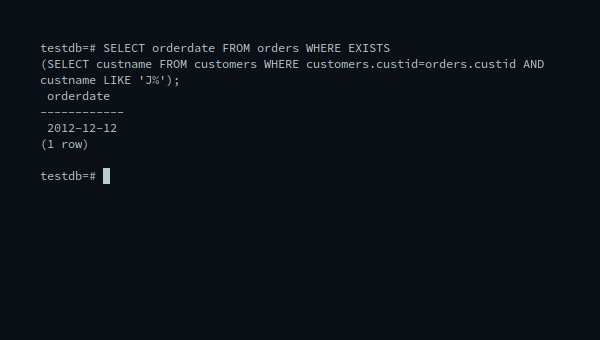
\includegraphics[width=\linewidth]{../Images/Joins/3.png}
\item Display the name and price of all items bought by the customer ‘Mickey’\newline
\begin{minted}{sql}

SELECT itemname, price FROM customers, items, orders, 
	WHERE orders.custid = customers.custid AND 
		  orders.itemid = items.itemid AND 
		  custname = 'Mickey';

\end{minted}
\newline
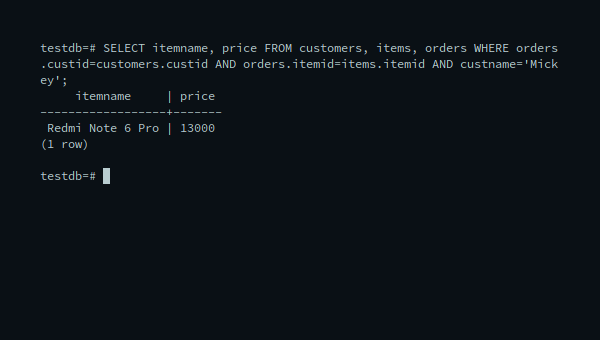
\includegraphics[width=\linewidth]{../Images/Joins/4.png}
\item List the details of all customers who have placed an order after January 2013 and not received delivery of items.\newline
\begin{minted}{sql}

SELECT * FROM customers WHERE custid IN 
	(SELECT custid FROM orders WHERE 
		orderdate > '01-JAN-2013' AND
		order id NOT IN 
			(SELECT orderid FROM delivery));

\end{minted}
\newline
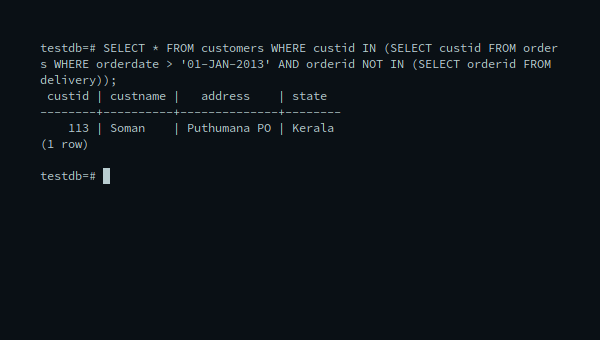
\includegraphics[width=\linewidth]{../Images/Joins/5.png}
\item Find the itemid of items which has either been ordered or not delivered. (Use UNION)\newline
\begin{minted}{sql}

SELECT itemid FROM orders WHERE EXISTS
	(SELECT orderid FROM orders) UNION
	SELECT orderid FROM delivery WHERE orderid NOT IN
	(SELECT orderid FROM delivery);

\end{minted}
\newline
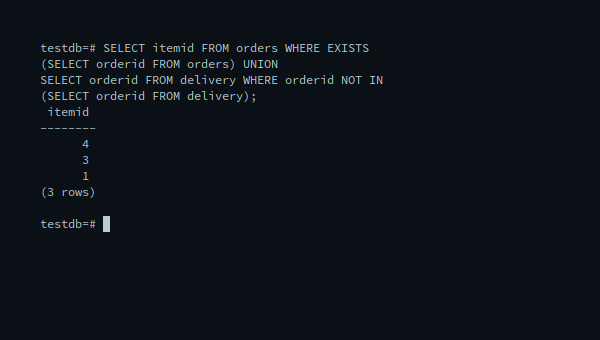
\includegraphics[width=\linewidth]{../Images/Joins/6.png}
\item Find the name of all customers who have placed an order and have their orders delivered.(Use SET INTERSECTION)\newline
\begin{minted}{sql}

SELECT custname FROM customers WHERE EXISTS
	(SELECT custid FROM orders WHERE 
		customers.custid = orders.custid)
	INTERSECT
	(SELECT custname FROM customers WHERE orderid IN
	(SELECT orderid FROM delivery));

\end{minted}
\newline
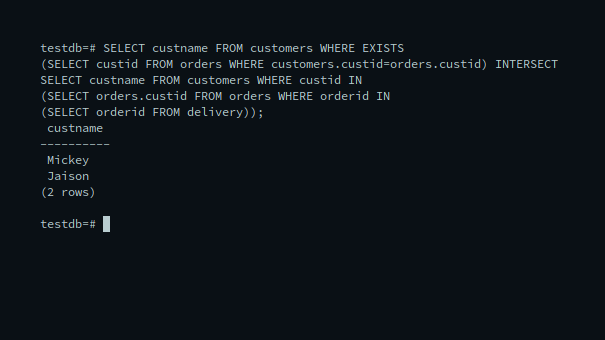
\includegraphics[width=\linewidth]{../Images/Joins/7.png}
\item Find the custname of all customers who have placed an order but not having their ordersdelivered. (Use SET MINUS)\newline
\begin{minted}{sql}

SELECT custname FROM customers WHERE custid IN 
	(SELECT custid FROM orders 
		EXCEPT SELECT custid FROM delivery);

\end{minted}
\newline
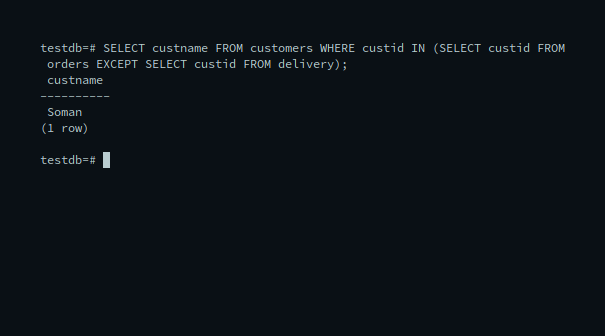
\includegraphics[width=\linewidth]{../Images/Joins/8.png}
\item Find the name of the customer who has placed the most number of orders.\newline
\begin{minted}{sql}

SELECT * FROM customers WHERE custid IN
	(SELECT custid FROM orders WHERE quantity IN
		(SELECT MAX(quantity) FROM orders));

\end{minted}
\newline
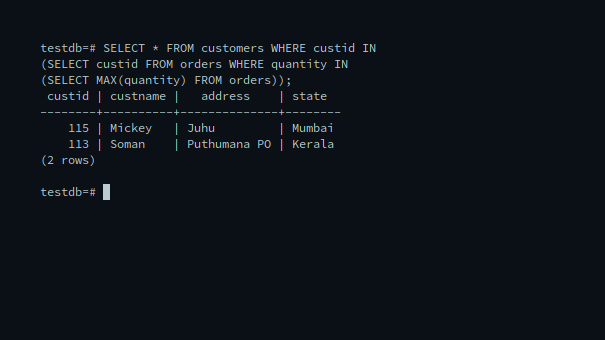
\includegraphics[width=\linewidth]{../Images/Joins/9.png}
\item Find the details of all customers who have purchased items exceeding a price of 5000\$.\newline
\begin{minted}{sql}

SELECT * FROM customers WHERE custid IN
	(SELECT custid FROM orders WHERE itemid IN
		(SELECT itemid FROM items 
			WHERE price > '5000'));

\end{minted}
\newline
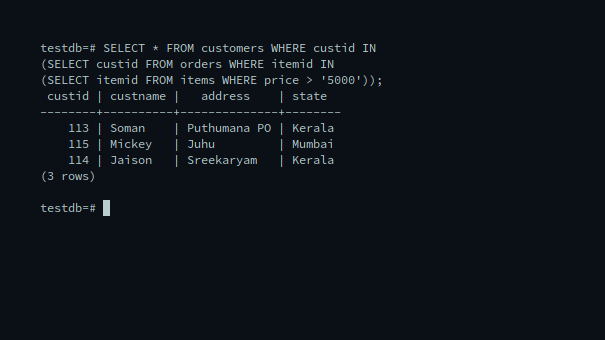
\includegraphics[width=\linewidth]{../Images/Joins/10.png}
\item Find the name and address of customers who has not ordered a 'Samsung Galaxy S4'\newline
\begin{minted}{sql}

SELECT custname, address FROM customers WHERE
custid NOT IN(
	SELECT custid FROM orders, items 
		WHERE items.itemname = 'Samsung Galaxy S4' AND
			  orders.itemid = items.itemid);

\end{minted}
\newline
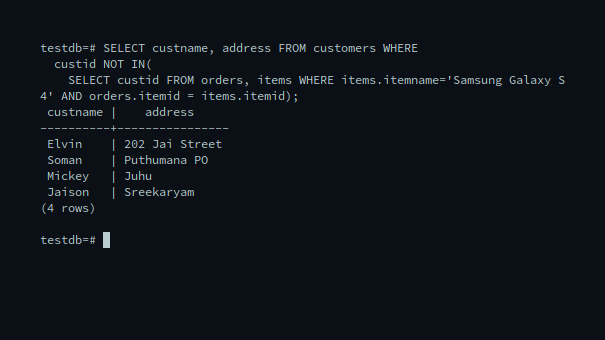
\includegraphics[width=\linewidth]{../Images/Joins/11.png}
\item Perform Left Outer Join and Right Outer Join on Customers & Orders Table.\newline
\begin{minted}{sql}

SELECT * FROM customers LEFT JOIN orders 
	ON customers.custid = orders.custid;

SELECT * FROM customers RIGHT JOIN orders 
	ON customers.custid = orders.custid;

\end{minted}
\newline
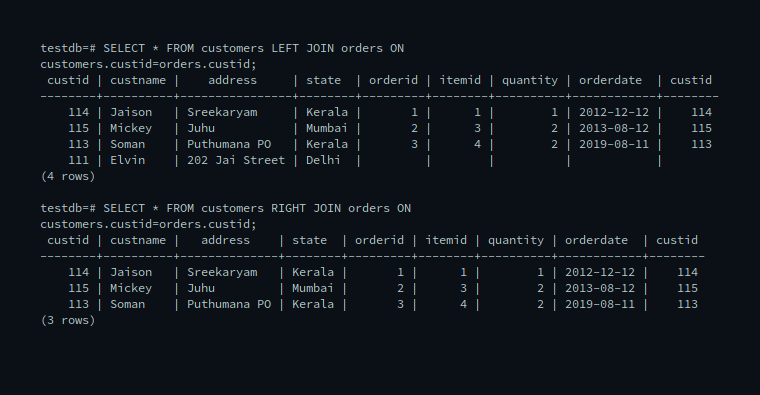
\includegraphics[width=\linewidth]{../Images/Joins/12.png}
\item Find the details of all customers grouped by state.\newline
\begin{minted}{sql}

SELECT state, COUNT(*) FROM customers 
	GROUP BY state;

\end{minted}
\newline
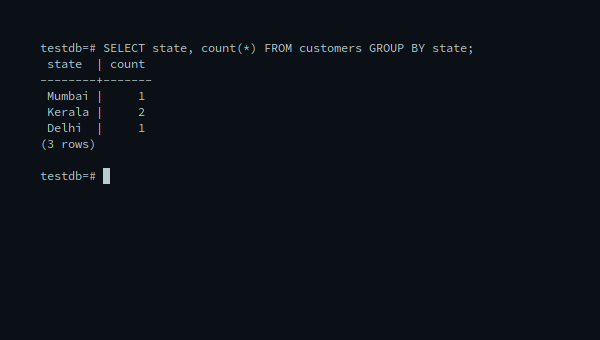
\includegraphics[width=\linewidth]{../Images/Joins/13.png}
\item Display the details of all items grouped by category and having a price greater than the average price of all items.\newline
\begin{minted}{sql}

SELECT itemid, itemname, category, price, instock 
	FROM items HAVING price > AVG(price);

\end{minted}
\newline
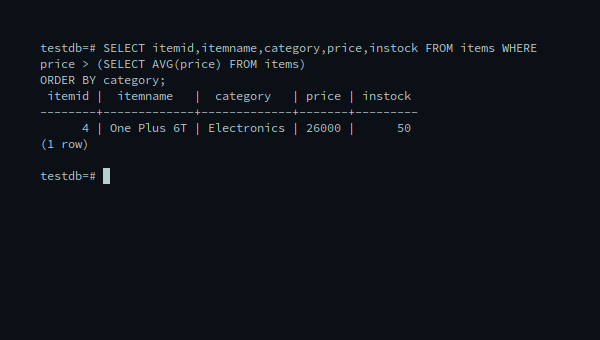
\includegraphics[width=\linewidth]{../Images/Joins/14.png}
\end{enumerate}

\section{Result}
Implemented the program for Join Statements, Set Operations, Nested Queries and Grouping using Postgresql 11.5 on Manjaro Linux and the output was obtained.